\documentclass[10pt, a4paper]{article}

%%% Packages %%%
\usepackage[margin=1in]{geometry} % Set margin size

\usepackage[utf8]{inputenc}
\usepackage[english]{babel}
\usepackage{amsmath}
\usepackage{amsfonts}
\usepackage{amssymb}
\usepackage{lmodern}
\usepackage{amsthm}
\usepackage{graphicx}

%%% Title page %%%
\title{CO495 - Coursework 1}
\author{Mehdi Bahri}
%\date{}

\newcommand{\R}{\mathbb{R}}
\newcommand{\CC}{\mathcal{C}}

\usepackage{fancyhdr}
\pagestyle{fancy}
\lhead{CO495 - Advanced Statistical Machine Learning}
\rhead{Coursework 1}

\begin{document}

\maketitle

\tableofcontents

\section{Description of the code}
We implemented the following algorithms in their respective MATLAB files.

\subsection{Generalities}
The different implementations all reside in the \texttt{Implem} folder, which should be added to MATLAB's path.

\subsection{PCA}
PCA is implemented in \texttt{pcomp.m}, \texttt{pcomp\_std.m} and \texttt{pcomp\_trick.m}.

\texttt{pcomp.m} is a wrapper around the two other files that implement two different strategies for computing PCA. Either the standard way by performing Eigen analysis on the covariance matrix (\texttt{pcomp\_std.m}) or by using the kernel trick (the covariance being a bilinear, symmetric, positive semi-definite application, it is close enough to a dot product and can be seen as the "canonical" kernel) in \texttt{pcomp\_trick.m}.

\texttt{pcomp.m} chooses automatically between the two strategies depending on the shape of the matrix to always perform Eigen analysis on the smallest possible matrix.

\subsection{Whitened PCA}

Whitened PCA can be obtained from \texttt{pcomp.m} by calling the function with arguments \texttt{pcomp(data, 'whiten', true)}.

\subsection{LDA}
Linear Discriminant Analysis (LDA) is implemented in \texttt{lda.m}.

\subsection{LPP}
We implemented Locality Preserving Projections in two different fashions that correspond to two different manners of computing the discrete Laplacian:

\paragraph{\texttt{lpp\_heat.m}} for heat kernel

Parameter \texttt{'t'} controls the constant used in the heat kernel (default $10^7$).

Parameter \texttt{center} allows choosing between LPP on centered or not-centered data. Default is centered.

\paragraph{\texttt{lpp\_knn.m}} for LPP with KNN.

The distance used for finding the K nearest neighbours can be controlled by passing \texttt{'distance', distance} as a parameter to the function. The default distance is the euclidean distance. We tried using the cosine distance as it is the one used by the code performing classification, but this distance gave worse results than euclidean. This can be explained by the fact that we perform classification on the low-dimensional space, whereas we compute the discrete Laplace-Beltrami operator on the original space.

The default number of nearest neighbours used is 10, but we tested different values in the range 5 to 150 and the number of neighbours seamed to have little impact in these particular cases. Parameter \texttt{'K'} controls the number of neighbours.

As with the heat kernel, our implementation centers the data by default but this can be disabled with the \texttt{center} parameter.

\subsection{FastICA}

We implented FastICA as described in the lectures notes and in the two original articles \footnote{Hyvarinen, A., "Fast and robust fixed-point algorithms for independent component analysis," in Neural Networks, IEEE Transactions on , vol.10, no.3, pp.626-634, May 1999
doi: 10.1109/72.761722} \footnote{A. Hyvärinen and E. Oja. 2000. Independent component analysis: algorithms and applications. Neural Netw. 13, 4-5 (May 2000), 411-430. DOI=http://dx.doi.org/10.1016/S0893-6080(00)00026-5 } by A. Hyvärinen but on the low-dimensional centered data obtained by performing whitened PCA.

This variation allows for faster computations than the original ICA that needs to be performed on the full covariance matrix. However, given that the only guarantee we get from ICA is that the output is \textit{uncorrelated}, and of low gaussianity; and that whitened PCA gives uncorrelated standardized data, we can question the usefulness of FastICA on this low-dimensional space.

Experimental results show FastICA performs worse than whitened PCA, so the two procedures are not equivalent.

FastICA is implemented in the file \texttt{fastica\_lowdim}, and the function accepts various optional parameters that are described in the code.

\newpage

\section{Results}

\subsection{YALE-B dataset}

In figure \ref{yaleb_all}, we present the performance of each algorithm on the YALE-B dataset plotted versus the number of dimensions we kept.

\begin{figure}[h!]
\centering
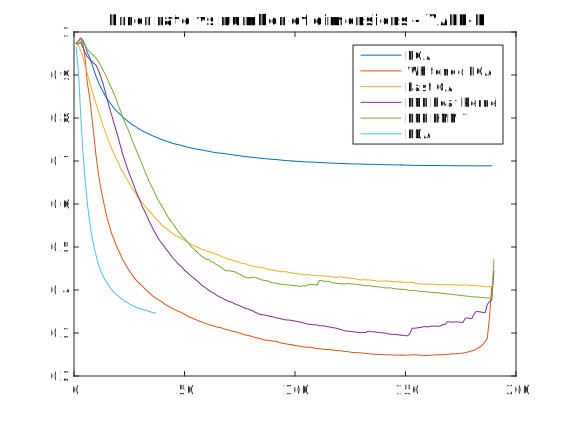
\includegraphics[width=0.75\textwidth]{yale/yale_all}
\caption{Comparative performance of the different algorithms on the YALE-B dataset}
\label{yaleb_all}
\end{figure}

\subsection{PIE dataset}
Similarly, figure \ref{pie_all} presents the comparative performances on the PIE dataset.
\begin{figure}[h!]
\centering
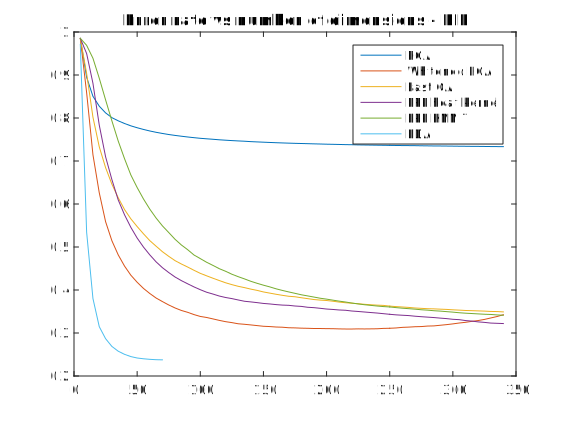
\includegraphics[width=0.75\textwidth]{pie/pie_all}
\caption{Comparative performance of the different algorithms on the PIE dataset}
\label{pie_all}
\end{figure}

\section{Discussion}

We compare the performance of the different algorithms. For LPP with KNN, we used 7 neighbours for computing the Laplacian.

We see that the general trend is that whitened PCA and LDA are the best performing algorithms.

PCA performs poorly, which is not surprising given the fact that it doesn't account for the difference in variance in the observations. The different face images all have different lightning conditions which induce differences in contrast.

This explains why whitened PCA performs much better than standard PCA, whitening the data ensures that a wide dynamic range in the images will not artificially give more importance to otherwise unimportant features.

LDA has the edge on the PIE dataset whereas it is less efficient than whitened PCA and LPP with a heat kernel on the YALE-B dataset. This could be explained by better-separated images in the PIE dataset that allow LDA to make tight highly separated clusters which can boost the performance of the KNN classifier we use.

On both datasets, the error using whitened PCA goes up beyond a given number of dimensions. This shows one major drawback of whitening the data: when every source of variability is given equal weight, then noise is equally important as actual features. This explanation is confirmed by the fact that the standard PCA does not exhibit the same behaviour.

On YALE-B, whitened PCA and LPP with both ways of computing the Laplacian show a steep spike in error when the last dimension is included. This might be that this dimension is pure noise, or is irrelevant and should have been dropped. This phenomenon does not arise on the PIE dataset so it is unlikely to be due to errors in the implementation.

ICA has average performance in both cases, this could be because independent components in images of faces are similar among classes. An intuitive view could be that independent component of faces could be, either anatomical parts such as a nose or eyes, or more abstract features such as borders. In both cases, we can imagine that these could be similar between people and therefore not very useful for classification.

The performance of LPP is higher than that of ICA. We can notice that LPP with KNN and 7 neighbours always seem to perform much worse than a heat kernel with $t = 10^7$.

On YALE-B, LPP achieves better results than LDA and follows the same trend as whitened PCA while being less efficient.

On PIE, LPP with KNN has an error rate that is decreasing, while LPP with heat kernel shows a slight increase than decreases again. The performance is worse than that of whitened PCA when few dimensions are kept, better for LPP with heat kernel when nearly all the dimensions are kept, and comparable to that of whitened PCA for LPP with KNN near the end of the spectrum. FastICA fares between LPP KNN and LPP heat intermediate numbers of dimensions.

\vspace{1em}

Figures \ref{compyale} and \ref{comppie} show the images obtained from the first three components returned by each algorithm and can help interpreting the results. Please note that the images have been scaled so they do not reflect the way PCA and whitened PCA handle contrast.

PCA is highly interpretable in the sense that each component can be used to reconstruct any of the faces, so they represent common features of all images and are close to actual face images.

The components obtained with the other algorithms are much more abstract. On YALE-B, most have little in common with the original face images, and this could explain why they perform poorly at classifying faces. This hypothesis is backed by the fact that on the PIE dataset, these components share a much neater common structure with the data.

LDA, which is the best-performing algorithms on PIE, seems to give especially useful components. The three components are structurally similar to faces, and seem to capture very well one given class as the three seem noticeably different from one another. This might show that the data points from one given class are well grouped within a class (similarity) and well separated between classes (differences between components).

\begin{figure}[h!]
\centering
\begin{tabular}{lccc}
PCA & \includegraphics{yale/yale_pca1} & \includegraphics{yale/yale_pca2} & \includegraphics{yale/yale_pca3} \\
Whitened PCA & \includegraphics{yale/yale_pca_white1} & \includegraphics{yale/yale_pca_white2} & \includegraphics{yale/yale_pca_white3} \\
LDA & \includegraphics{yale/yale_lda1} & \includegraphics{yale/yale_lda2} & \includegraphics{yale/yale_lda3} \\
LPP Heat & \includegraphics{yale/yale_lpp_heat1} & \includegraphics{yale/yale_lpp_heat2} & \includegraphics{yale/yale_lpp_heat3} \\
LPP Heat & \includegraphics{yale/yale_lpp_knn1} & \includegraphics{yale/yale_lpp_knn2} & \includegraphics{yale/yale_lpp_knn3} \\
FastICA & \includegraphics{yale/yale_ica1} & \includegraphics{yale/yale_ica2} & \includegraphics{yale/yale_ica3} \\
\end{tabular}
\caption{First 3 components obtained on the YALE-B dataset for each algorithm}
\label{compyale}
\end{figure}


\begin{figure}[h!]
\centering
\begin{tabular}{lccc}
PCA & \includegraphics{pie/pie_pca1} & \includegraphics{pie/pie_pca2} & \includegraphics{pie/pie_pca3} \\
Whitened PCA & \includegraphics{pie/pie_pca_white1} & \includegraphics{pie/pie_pca_white2} & \includegraphics{pie/pie_pca_white3} \\
LDA & \includegraphics{pie/pie_lda1} & \includegraphics{pie/pie_lda2} & \includegraphics{pie/pie_lda3} \\
LPP Heat & \includegraphics{pie/pie_lpp_heat1} & \includegraphics{pie/pie_lpp_heat2} & \includegraphics{pie/pie_lpp_heat3} \\
LPP KNN (7) & \includegraphics{pie/pie_lpp_knn1} & \includegraphics{pie/pie_lpp_knn2} & \includegraphics{pie/pie_lpp_knn3} \\
FastICA & \includegraphics{pie/pie_ica1} & \includegraphics{pie/pie_ica2} & \includegraphics{pie/pie_ica3} \\
\end{tabular}
\caption{First 3 components obtained on the PIE dataset for each algorithm}
\label{comppie}
\end{figure}
\end{document}
